\subsection{When does scene adaptation help? Four scenes and five mitigations}
\label{sec:adapt}
\ifHaveMultiscene
\textbf{Adaptation to one camera hurts every other camera.} Fig.~\ref{fig:transfer} and Table~\ref{tab:adapt} extend
the held-out test to all four scenes and to human-labelled COCO people. Fine-tuning \yolo{} on aa1 raises aa1 \AP{}
from \MsPtAa{} to \MsFtAa{} but lowers it on \emph{every} other scene: scene~1 \MsPtVone{}$\rightarrow$\MsFtVone,
scene~2 \MsPtVtwo{}$\rightarrow$\MsFtVtwo, held-out \MsPtHo{}$\rightarrow$\MsFtHo, and on COCO people from
\MsPtCoco{} to \MsFtCoco{}: the student forgets what a person looks like outside aa1. Adapting to one campus scene
instead shows the same pattern: each single-scene model improves its own scene over the pretrained model and is worse
than the pretrained model on every other scene and on COCO. The fine-tuned \rfdetr, in contrast, improves on its pretrained weights on the campus scenes
(\MsRfFtVone{} and \MsRfFtVtwo{} vs.\ \MsRfPtVone{} and \MsRfPtVtwo) and loses little on COCO
(\MsRfFtCoco{} vs.\ \MsRfPtCoco). Training on three scenes helps the scenes included and partly the unseen one
(held-out \MsMultiHo{} vs.\ \MsFteHo{} for aa1 alone), but stays below the pretrained model (\MsPtHo).

\figif{fig_transfer.pdf}{%
\begin{figure}[t]
\centering
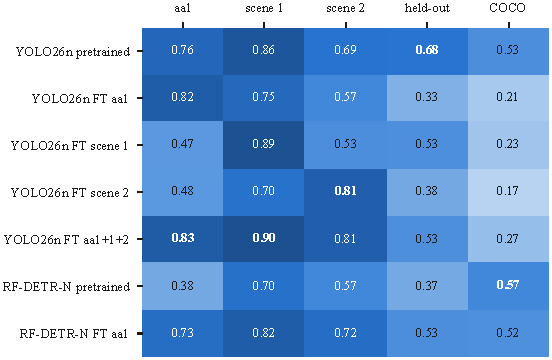
\includegraphics[width=\columnwidth]{figures/fig_transfer.pdf}
\caption{Cross-scene transfer: \AP{} of each training configuration (rows) on each test scene (columns); bold: best
per column. Single-scene fine-tuning of \yolo{} wins its own scene and loses everywhere else, including COCO.}
\label{fig:transfer}
\end{figure}}

\ifHaveLabelThr
\textbf{Why small people disappear: the label threshold.} A single 0.40 cut on the fused teacher score is not neutral
with respect to size. Of the teacher boxes ($s\ge0.15$) on the aa1 training frames, \LtAaA{} of those under 32\,px
tall and \LtAaB{} of those 32--64\,px tall fall below the cut, against \LtAaD{} at 128--256\,px and \LtAaE{} above
256\,px; the held-out video shows the same profile (\LtHoA, \LtHoB, \LtHoD, \LtHoE). A person left out of the labels
is not ``unknown'' to the student but \emph{background}, so fine-tuning is trained to suppress exactly the small, far
people whose recall collapsed on the held-out video (Sec.~\ref{sec:heldout}). Some of the low-score boxes are not
people, so the profile alone is not proof; the \emph{ignore} variant tests it causally by removing these
\LtGreyed{} uncertain regions from the training images instead of treating them as background.
\fi


\begin{table*}[t]
\centering
\caption{Scene adaptation and its mitigations: \AP{} per scene (aa1 = adaptation scene; scenes 1 and 2 = other campus
cameras; held-out = test1, never used for any choice; COCO = 600 human-labelled COCO val2017 images). Last columns:
recall of people 32--64\,px tall and false positives per frame on the held-out video, at each model's frozen
threshold. $^\dagger$Trained on scenes 1 and 2, so those columns are in-domain.}
\label{tab:adapt}
\footnotesize
\setlength{\tabcolsep}{4pt}
\begin{tabular}{lccccc|cc}
\toprule
Training / model & aa1 & scene 1 & scene 2 & held-out & COCO & $R_{32\text{--}64}$ & FPPI \\
\midrule
\yolo{} pretrained & \MsPtAa & \MsPtVone & \MsPtVtwo & \MsPtHo & \MsPtCoco & \MsPtHoSmall & \MsPtHoFppi \\
\midrule
FT-aa1 (submitted, 1-class head) & \MsFtAa & \MsFtVone & \MsFtVtwo & \MsFtHo & \MsFtCoco & \MsFtHoSmall & \MsFtHoFppi \\
FT-aa1 (80-class head, reference) & \MsFteAa & \MsFteVone & \MsFteVtwo & \MsFteHo & \MsFteCoco & \MsFteHoSmall & \MsFteHoFppi \\
\quad WiSE, $\alpha{=}\WiFteRawAlpha$ (aa1+COCO val) & \MsWiFtAa & \MsWiFtVone & \MsWiFtVtwo & \MsWiFtHo & \MsWiFtCoco & \MsWiFtHoSmall & \MsWiFtHoFppi \\
\quad WiSE, shift-aware matrix choice & \MsSelAa & \MsSelVone & \MsSelVtwo & \MsSelHo & \MsSelCoco & \MsSelHoSmall & \MsSelHoFppi \\
\midrule
FT-aa1 + COCO replay & \MsRepAa & \MsRepVone & \MsRepVtwo & \MsRepHo & \MsRepCoco & \MsRepHoSmall & \MsRepHoFppi \\
FT-aa1, frozen backbone & \MsFrzAa & \MsFrzVone & \MsFrzVtwo & \MsFrzHo & \MsFrzCoco & \MsFrzHoSmall & \MsFrzHoFppi \\
FT-aa1, uncertain boxes ignored & \MsIgnAa & \MsIgnVone & \MsIgnVtwo & \MsIgnHo & \MsIgnCoco & \MsIgnHoSmall & \MsIgnHoFppi \\
\midrule
FT aa1+scene 1+scene 2$^\dagger$ & \MsMultiAa & \MsMultiVone & \MsMultiVtwo & \MsMultiHo & \MsMultiCoco & \MsMultiHoSmall & \MsMultiHoFppi \\
\quad WiSE, $\alpha{=}\WiMultiRawAlpha$$^\dagger$ & \MsWiMuAa & \MsWiMuVone & \MsWiMuVtwo & \MsWiMuHo & \MsWiMuCoco & \MsWiMuHoSmall & \MsWiMuHoFppi \\
\midrule
\rfdetr{} FT-aa1 @640 & \MsRfFtAa & \MsRfFtVone & \MsRfFtVtwo & \MsRfFtHo & \MsRfFtCoco & \MsRfFtHoSmall & \MsRfFtHoFppi \\
\rfdetr{} FT-aa1, tested @1280 & \MsRfFtHiAa & \MsRfFtHiVone & \MsRfFtHiVtwo & \MsRfFtHiHo & \MsRfFtHiCoco & \MsRfFtHiHoSmall & \MsRfFtHiHoFppi \\
\bottomrule
\end{tabular}
\end{table*}

\textbf{Mitigations.} All variants share the reference recipe and change one thing (Sec.~\ref{sec:variants}).
\emph{Weight-space ensembling} is the most effective and costs nothing: blending the pretrained and fine-tuned
weights keeps most of the in-domain gain while restoring transfer (Fig.~\ref{fig:tradeoff}); with $\alpha$ chosen on
aa1-valid and COCO-val (\WiFteRawAlpha) the blend scores \MsWiFtAa{} on aa1 and \MsWiFtHo{} on the held-out video,
where it beats \emph{both} endpoints, and the path lies far above the straight line between the endpoints, i.e.\ it is
effectively robust in the sense of~\cite{taori2020shift}. Re-estimating the BatchNorm statistics after blending, the
usual advice for merged networks, \emph{hurt}: in-domain at every $\alpha$, and on the held-out video for all but
the blends closest to the fine-tuned model (\WiFteBnHo{} at its validation-chosen $\alpha{=}\WiFteBnAlpha$); 192
calibration images estimate the statistics worse than interpolating two well-estimated sets. \emph{COCO replay} gives the best in-domain single model (\MsRepAa) and recovers much of the held-out
loss (\MsRepHo; COCO \MsRepCoco). A \emph{frozen backbone} keeps the pretrained features (held-out \MsFrzHo, COCO
\MsFrzCoco) and has the fewest false positives on the held-out video (\MsFrzHoFppi{} per frame vs.\ \MsFteHoFppi). The
\emph{ignore} variant raises held-out \AP{} over the same-recipe reference (\MsIgnHo{} vs.\ \MsFteHo) but leaves COCO
forgetting unchanged (\MsIgnCoco) and moves the valid-optimal threshold to \MsIgnConf, so the label threshold explains
part of the small-person loss while forgetting of general person features explains more. More scenes plus WiSE
($\alpha{=}\WiMultiRawAlpha$) gives the best held-out \yolo{} (\MsWiMuHo). The submitted 1-class model and the
80-class reference behave alike in-domain (\MsFtAa, \MsFteAa) but the latter forgets more (held-out \MsFteHo).

\figif{fig_tradeoff.pdf}{%
\begin{figure*}[t]
\centering
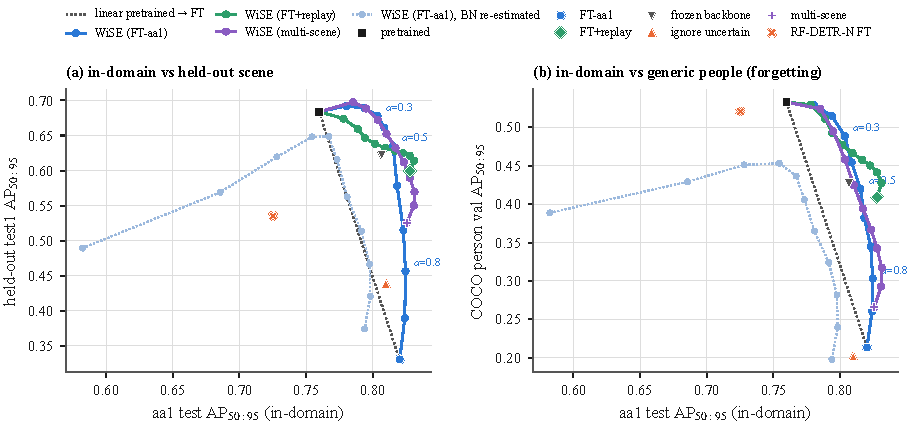
\includegraphics[width=\textwidth]{figures/fig_tradeoff.pdf}
\caption{Adaptation trade-offs. WiSE paths run from $\alpha{=}0$ (the pretrained model, black square) to
$\alpha{=}1$ (the fine-tuned model). Points above the dotted pretrained$\rightarrow$fine-tuned line are more robust
than the linear trend. (a)~In-domain vs.\ held-out camera; (b)~in-domain vs.\ COCO people (forgetting).}
\label{fig:tradeoff}
\end{figure*}}

\ifHaveTrackVone
\textbf{Tracking on longer, unseen videos.} With every parameter frozen from aa1, ByteTrack on the two 200\,s campus
videos (\StVoneGtIds{} and \StVtwoGtIds{} pseudo-GT identities) repeats the detection picture
(Table~\ref{tab:scenetrack}): the fine-tuned \rfdetr{} tracks best on both and the fine-tuned \yolo{} worst; on
scene~1 the fine-tuned \yolo{} also recovers far fewer counting-line events (crossing F1 \StVoneFtCrossFone{} vs.\
\StVoneRfFtCrossFone{} and \StVonePtCrossFone), while on scene~2, where people are large and close, all three are
similar. The aa1-tuned tracker parameters beat ByteTrack's defaults on both unseen videos for both fine-tuned
detectors, so the \GridSize-configuration search on 15\,s did not merely fit that window.
\begin{table}[t]
\centering
\caption{ByteTrack on the 200\,s campus videos, parameters frozen from aa1 (defaults in parentheses); crossings: F1
of matched counting-line events ($\pm$1\,s, same direction).}
\label{tab:scenetrack}
\scriptsize
\setlength{\tabcolsep}{2.2pt}
\begin{tabular}{lcc|cc}
\toprule
 & \multicolumn{2}{c|}{scene 1} & \multicolumn{2}{c}{scene 2} \\
Detector & HOTA & Cross.\ F1 & HOTA & Cross.\ F1 \\
\midrule
\yolo{} FT-aa1 & \StVoneFtHota{} (\StVoneFtHotaDef) & \StVoneFtCrossFone & \StVtwoFtHota{} (\StVtwoFtHotaDef) & \StVtwoFtCrossFone \\
\rfdetr{} FT-aa1 & \StVoneRfFtHota{} (\StVoneRfFtHotaDef) & \StVoneRfFtCrossFone & \StVtwoRfFtHota{} (\StVtwoRfFtHotaDef) & \StVtwoRfFtCrossFone \\
\yolo{} pretrained & \StVonePtHota{} (\StVonePtHotaDef) & \StVonePtCrossFone & \StVtwoPtHota{} (\StVtwoPtHotaDef) & \StVtwoPtCrossFone \\
\bottomrule
\end{tabular}
\end{table}
\fi

\textbf{Practical rule.} Single-camera pseudo-label fine-tuning of a compact detector should not be deployed on
other cameras as is. A WiSE blend, chosen on validation data from \emph{other} cameras, keeps most of the
adaptation gain where it was trained and the pretrained robustness elsewhere, at zero training or inference cost;
replay or a frozen backbone are the training-time alternatives.
\else
Multi-scene results are pending.
\fi
